\chapter{Evaluation}

In this chapter we describe the different tasks (minigames) our agent is evaluated in, list the results the agent has obtained and provide commentary on how these results compare to the expectations and human expert benchmarks.

\section{Tasks}

Each evaluated task is a StarCraft II minigame: a map with some simple pre-defined MDP. These minigames are meant to test agents ability to learn and generalize across different environments.
\\\\
\textbf{MoveToBeacon} map requires the agent to navigate a single unit to a beacon -- a specific location on the map, identified by a large green circle.
\\\\
In \textbf{CollectMineralShards} map the agent has to collect mineral shards (resource nodes) by walking on top of them. The map provides the agent with two units and an optimal strategy would be to navigate them simultaneously.
\\\\
\textbf{DefeatRoaches} map introduces static opponent army units, which the agent has to defeat with his own. Opponent and agent units are significantly different, so the agent has to learn the characteristics of both types while only controlling its own units.
\\\\
\textbf{DefeatBanelingsAndZerglings} map expands on the adversarial objective by providing opponent with two types of units: Zerglings and Banelings. The Baneling units can explode on contact with their opponents, meaning that the agent has to learn precise navigation and avoidance mechanisms in order to succeed.
\\\\
\textbf{FindAndDefeatZerglings} map tests agents' ability to navigate in a partially observable environment. An agent has to find and defeat opponent units scattered across the map.
\\\\
\textbf{CollectMineralsAndGas} map objective is to test agents economic reasoning capabilities. The only goal of the map is to gather as many resources as possible, though there are multiple paths to achieving this goal, including building additional workers and a secondary base to speed up their gathering rate. 
\\\\
\textbf{BuildMarines} is similar to previous map, except the objective is to build as many units of a specific type (Marine) as possible. The path to building these units requires completion of multiple sub-tasks with long time-steps inbetween. This, in turn, tests agent's long term planning capabilities.

\section{Setup}

Choice of hyperparameters such as learning rate, loss weights and batch size is typically made by repeatedly randomly sampling from some expected interval and training to a stable policy until satisfying results are achieved. Unfortunately this approach is not feasible for the StarCraft II environment as the agent might take significant amount of time before it is clear whether hyperparameter choice was good. Furthermore, even with fixed hyperparameters the end result varies wildly across different seeds. For this reason many hyperparameters were chosen based on the initial performance of the agent on a subset of maps and locked for future experimentation.
\\\\
Screen and minimap resolution of presented results was locked to 16px for all map environments. For comparison, DeepMind used 64px resolutions. The choice for lower resolution is driven purely by time constraints, as computational requirements grow significantly with higher resolutions (about 25x increase in wall clock time requirements for 64px). Agents capacity for learning in higher resolutions to the level of presented results was empirically verified at least once for every map. On some of the maps with higher resolution agents training speed improved in terms of number of samples required to reach the target results, but was unfortunately too slow in terms of wall clock time.
\\\\
While the codebase was developed with dynamic configuration of input features in mind, they were locked across all map environments during results gathering phase to ensure that the agent is capable of generalizing -- learning complex policies across varying environments.
\\\\
Optimization algorithm was chosen between Adam~\cite{Kingma2014} and RMSProp~\cite{Tieleman2012}, two SGD improvements. RMSProp was used for all minigames except \texttt{FindAndDefeatZerglings}, where Adam was used instead. Adam is considered to be the best algorithm in supervised learning scenario, where its momentum build up helps jump through unfavorable local optima. For this same reason we have considered Adam to be unfavorable in RL scenarios as the input data distribution is inherently not stationary and thus momentum build up may be detrimental to agents performance. Surprisingly it has significantly surpassed RMSProp on the \texttt{FindAndDefeatZerglings} minigame, perhaps due to the unique partially observable nature of the map.
\\\\
All model weights were initialized with He initialization~\cite{He2015}, which is shown to produce better results than the alternatives (eg. uniform or normal) and has become standard practice in modern Machine Learning. 

\section{Results}

Results were collected by first training implemented agent until its average score matches baseline results and then executing in test mode, similarly to the training mode. The agent operates in 32 environments and the average score over those 32 runs is reported as the final result. If target score is not achieved in reasonable time then the training is prematurely terminated. Time limit depends on the minigame, from 30 minutes for MoveToBeacon to 50 hours for FindAndDefeatZerglings (wall clock time). To ensure that our agent is capable of converging to a policy with target results, we run training procedure four times with different random seeds. Results are summarized in the table~\ref{tab:results} below.
\\\\
Note that our method is different from how DeepMind has gathered their results, where they launched 100 instances with different hyperparameter sets for 500 million frames and chose best out of them. This method was not chosen due to unrealistic computational requirements: obtaining results presented in this work took about 25,000 CPU hours in total, which means that repeating DeepMind experiments in full would take over 5,000,000 CPU hours.

\begin{table}[h]
\centering
\begin{tabular}{| l | l | l | l |}
\hline
\bf{Map Name} & \bf{A2C Agent} & \bf{DeepMind} & \bf{Human} \\
\hline
MoveToBeacon & 26.3 $\pm$ 0.5 & 26 & 28 \\
\hline
CollectMineralShards & 106 $\pm$ 4.3 & 103 & 177 \\
\hline
DefeatRoaches & \textbf{147} $\pm$ 38.7 & 100 & 215 \\
\hline
DefeatBanelingsAndZerglings & \textbf{230} $\pm$ 106.4 & 62 & 727 \\
\hline
FindAndDefeatZerglings & 43 $\pm$ 5 & 45 & 61 \\
\hline
CollectMineralsAndGas & 3340 $\pm$ 185 & 3978 & 7566 \\
\hline
BuildMarines & 0.55 $\pm$ 0.25 & 3 & 133 \\
\hline
\end{tabular}
\caption{Mean and std.dev of total reward for an episode of the implemented agents relative to DeepMind benchmarks. ``A2C Agent'' stands for our baseline implementation, ``DeepMind'' for DeepMind's baseline FullyConv results and ``Human'' for DeepMind's GradMaster ranked expert results.}
\label{tab:results}
\end{table}

\section{Discussion}

Our agent matches or slightly surpasses DeepMind FullyConv baseline results on most of the maps. A video of our agent navigating given set of maps has been recorded and available online: \url{https://youtu.be/gEyBzcPU5-w}
\\\\
\textbf{MoveToBeacon} map can be considered solved, 2 point difference from human expert is most likely due to luck in random placements of the beacon. Specifically on this map the agent learned optimal policy very suddenly: behavior seemed quite random for majority of the time with optimal actions emerging almost instantly after first few good attempts.
%\begin{figure}[!ht]
%\begin{center}
%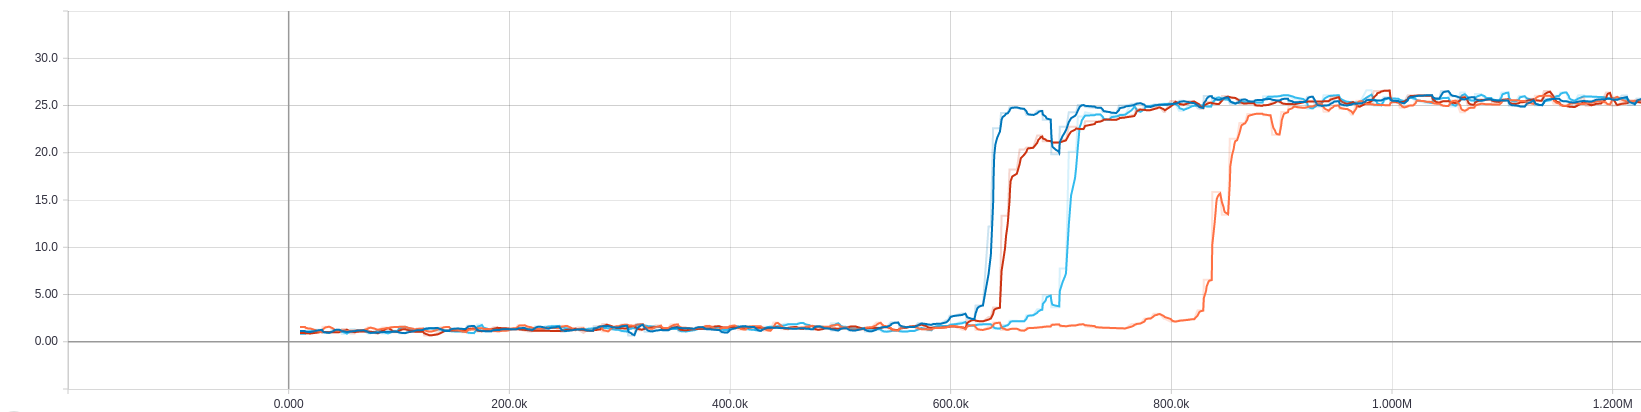
\includegraphics[width=\textwidth]{results/MoveToBeacon}
%\caption{MoveToBeacon results. Episode cumulative reward on y-axis and number of samples on x-axis.}
%\label{fig:res/beacon}
%\end{center}
%\end{figure}
%\noindent 
\\\\
\textbf{CollectMineralShards} map matches DeepMind baseline results, but is almost two times worse than human expert.
The environment contains two units that could be controlled at almost the same time, singificantly increasing the speed of gathering the shards. Seems that the agent is unable to discover this strategy.
\\\\
\textbf{DefeatRoaches} map matches DeepMind baseline results, but is two times worse than human expert.
Most likely optimal strategy is to defeat opponent army in parts by getting attention of a subset at a time.
\\\\
\textbf{DefeatBanelingsAndZerglings} results are better than DeepMind's baseline, but significantly worse than human benchmark.
This map requires precise control of the individual units in the army in order to minimize damage from baneling explosions and the agent fails to learn anything more advanced than some initial splits. We observe significant variance of results in this minigame, most likely stemming from its volatile nature.
\\\\
\textbf{FindAndDefeatZerglings} results match DeepMind baseline, but are worse than human expert. Most likely reason is that since the map is not fully visible, a human expert can remember where enemy army can be located on the map, whereas best policy our agent has discovered is to just move the units in a trajectory that covers the full map.
\\\\
\textbf{CollectMineralsAndGas} results are slightly below DeepMind baseline and more than two times worse than human expert. The "optimal" strategy our agent has learned is to simply send the initial workers to gather resources and wait for the remaining time. Judging by DeepMind results, their agents strategy is similar with maybe 1 more worker produced.
\\\\
\textbf{BuildMarines} map proved to be too difficult for our agent to learn any reasonable policy on. Judging by relative score, this seems to be true for DeepMind agent as well. As this map requires long-term economic planning, solving it is most likely too difficult without some sort of temporal structure such as LSTM~\cite{Hochreiter1997}.

\subsection{Failures}

In this section we list alternative choices (either architectural or in agent setup) that were considered failures due to agents poor performance.
\\\\
Although the SC2LE paper only mentions embedding into continuous space, we have also experimented with having dimensionality reduced to a different space size. The size was either fixed to a small number (ex. 2 or 3) or dynamically changed based on the feature (ex. $\log_2(D)$, where $D$ is number of categorical levels). In the end results were not consistently better than simply using continuous space.
\\\\
We have experimented with an alternative approach to embedding categorical spatial data described in section 2.1.1. While the main approach requires defining a separate embedding layer for every categorical feature, an alternative solution would be to combine all categorical spatial inputs into a single $H \times W \times \big (\sum C_i \big)$ tensor, where $C_i$ defines number of categorical levels of i-th feature. In theory this approach had two benefits: ease of implementation and computation (can run a single convolutional operation for all categorical features at the same time) and the potential for learning interactions of different features since they all influenced each others output filters. However, empirically this lead to very unstable learning trajectory, often times oscillating between reasonable policies and borderline random behavior.
\\\\
Singificant amount of time was spent investigating influence of various input features on agents speed of convergence to target results. While we have found some configurations that led to as much as 10x improvement in learning speed on some of the maps, they typically resulted in worse perfomance on other maps.

\subsection{Future Work}
% TODO Alpha-Zero like approach?
Possible direction for future work could in investigating ways of improving sample efficiency of the agent (number of samples required to achieve target results), either by applying alternative algorithms such as PPO, ACKTR or SAC, or applying variance reduction techniques from Monte Carlo methods such as Antithetic Variates. 
\\\\
A promising direction to explore would be to pre-train agent model in a supervised learning setting with data gathered from human experts.
\\\\
An alternative direction could be in exploring Hierarchical Reinforcement Learning -- a way to organize agents tasks into hierarchies. While the goal is to produce an agent capable of beating a professional human player in a modern video game such as StarCraft II, but solution to this task is still an open research question, potentially many years away.